%% PREAMBLE %%

\documentclass{beamer}

\usepackage[english]{babel}
\usepackage[utf8]{inputenc}
\usepackage{amssymb}
\usepackage{graphics}
\usepackage{times}
\usepackage{textpos}
\usepackage{pgf}
\usepackage{enumerate}
\usepackage{xcolor}
\usefonttheme{serif}
\usepackage{csvsimple}
\usepackage{datatool}
\usepackage{natbib}
\usepackage{multirow}


% for circling significant regression table results
% option 1 use \cellcolor{colorname} to set cell color within table
\usepackage{color, colortbl} % here, use \rowcolor{colorname} to set row color
\definecolor{neonyellow}{RGB}{243,243,21}


% Theme Customization
% colors
\definecolor{GCblue}{RGB}{0,101,153}
\definecolor{GClblue}{RGB}{184,224,245}
\setbeamercolor{title}{fg=GCblue}
\setbeamercolor{frametitle}{fg=GCblue}
\setbeamercolor{structure}{fg=GCblue}
\setbeamercolor{headline}{fg=white,bg=GCblue}
\setbeamercolor{footline}{fg=GCblue}

% blocks
\setbeamercolor{block title}{fg=white,bg=GCblue}
\setbeamercolor{block title example}{fg=GCblue,bg=GClblue}
\setbeamercolor{block body example}{fg=black,bg=GClblue}

% figures/tables
\setbeamertemplate{caption}[numbered]

% outer/inner themes
\setbeamertemplate{items}[triangle]
\setbeamertemplate{blocks}[rounded][shadow=true] 
\setbeamertemplate{navigation symbols}{} 
\setbeamertemplate{headline}
	{% 
		\begin{beamercolorbox}{headline}
		\vskip3pt\makebox[4cm][c]{THE GRADUATE CENTER, CUNY}
		\hfill\makebox[4cm][c]{PhD PROGRAM in ECONOMICS}
		\vskip3pt
		\end{beamercolorbox}%
	}
\setbeamertemplate{footline}
	{	\hfill\rule{11.7cm}{.1mm}
		\vskip3pt
		\hfill\insertauthor \ --  \insertshorttitle \ -- \insertdate {  }%
		\ -- {Slide } \insertframenumber / \inserttotalframenumber {  }
		\vskip3pt
	}	
\logo{\pgfputat{\pgfxy(-12.1,-.55)}{\pgfbox[center,base]%
	{
\includegraphics[width=.8cm]{gclogo2.pdf}}}} 
	 
% Title Page Elements
\title[SHORT TITLE]{ENTER TITLE HERE}
\subtitle{ENTER SUBTITLE HERE}
\author{ENTER NAME HERE}
\institute[The Graduate Center, CUNY]{PhD Program in Economics\\
	The Graduate Center, City University of New York}

%\beamerdefaultoverlayspecification{<+->}

\begin{document}

%-------------------------------------------------------------------------------------------
%-------------------------------------------------------------------------------------------
{
\setbeamertemplate{background canvas}{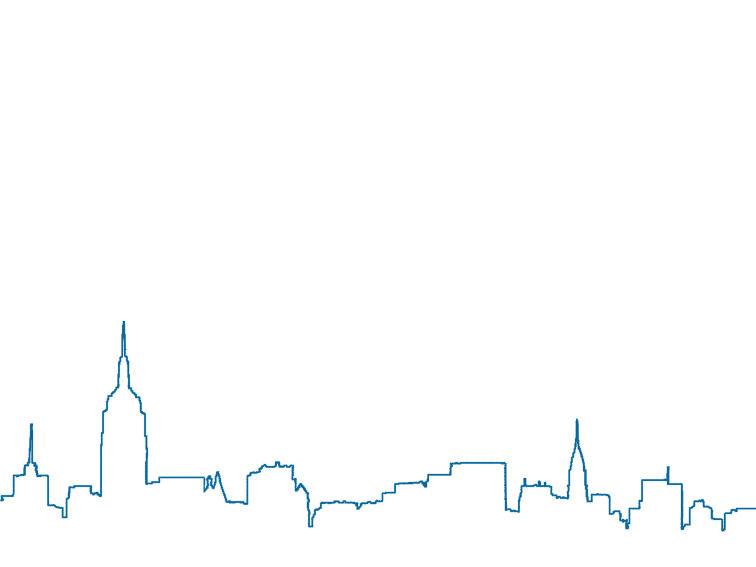
\includegraphics{skyline4.pdf}} 
\setbeamertemplate{footline}
	{	\hrule	
		\vskip3pt
		\hfill\insertdate {  }
		\vskip3pt
	}
\logo{}	
\begin{frame} 
 \titlepage
\end{frame} 
} 
%-------------------------------------------------------------------------------------------
%-------------------------------------------------------------------------------------------
\begin{frame}{Outline}





\end{frame}
%-------------------------------------------------------------------------------------------
%-------------------------------------------------------------------------------------------
%\begin{frame}{References}
 
%\footnotesize
% or insert [allowframebreaks] before frame title

%\bibliographystyle{apa-good}
%\bibliography{econ2}			

%\end{frame}
%-------------------------------------------------------------------------------------------
%-------------------------------------------------------------------------------------------




\end{document}

